\documentclass[11pt]{article}

\usepackage[margin=1in]{geometry}
\usepackage{amsmath,amsthm,amsfonts}
\usepackage[utf8]{inputenc}
\usepackage{amssymb}
\usepackage[mathscr]{eucal}
\usepackage{graphicx}
\usepackage{listings}
\usepackage{titlesec}
\usepackage{tikz}
\usepackage{xcolor}
\usepackage[OT1]{fontenc}
\usepackage{physics}
\usepackage{xpatch}

\usetikzlibrary{graphs}
\usetikzlibrary{graphs.standard}

\setlength\parindent{0pt}

\newtheoremstyle{dotless}{}{.5\topsep}{\itshape}{}{\bfseries}{}{ }{}

\newtheoremstyle{dotles}{}{}{\upshape}{}{\bfseries}{}{ }{}

\theoremstyle{definition}
\newtheorem*{defin}{DEF}

\theoremstyle{dotles}
\newtheorem{innercustomex}{EX}
\newenvironment{exercise}[1]
  {\renewcommand\theinnercustomex{#1}\innercustomex}
  {\endinnercustomex}

\theoremstyle{dotless}
\newtheorem{proposition}{PROP}[section]

\theoremstyle{remark}
\newtheorem*{remark}{Remark}
\newtheorem{example}{Example}

\usepackage{hyperref}
\hypersetup{colorlinks=false}

\titleformat{\section}
{\normalfont\Large\bfseries}{\S\thesection.}{1em}{}



\begin{document}

\section{Fundamental Concepts}

\begin{defin}
A \textbf{graph} $G$ is a triple $(V(G),E(G),f)$ where $V(G)$ is the vertex set, $E(G)$ is the edge set, and $f$ associates two vertices with each edge. A \textbf{subgraph} $H$ of $G$ is a graph such that $V(H)\subseteq V(G)$, $E(H)\subseteq E(G)$, and $f_H=f$. A \textbf{decomposition} of a graph is a list of subgraphs such that each edge appears exactly once in each subgraph.\medbreak
Endpoints are \textbf{adjacent} if they are endpoints of a same edge. A \textbf{clique} in a graph is a set of pairwise adjacent vertices. An \textbf{independent set} in a graph is a set of pairwise non-adjacent vertices. A graph $G$ is \textbf{$k$-partite} if $V(G)$ can be expressed as the union of $k$ independent sets (\textbf{partite sets}). The \textbf{chromatic number} $\chi(G)$ of $G$ is the minimum number of colors needed to label the vertices so that adjacent vertices receive different colors. Vertex $v$ and edge $e$ are \textbf{incident} if $v$ is the endpoint of $e$. The \textbf{degree} of $v$ is the number of incident edges. \textbf{Isolated vertex} has vertex degree 0.\medbreak
A graph is \textbf{simple} if it has no loops or multiple edges (edges having the same pair of endpoints). The \textbf{complement} $\overline{G}$ of simple graph $G$ is the simple graph with vertex set $V(G)$ and $uv\in E(\overline{G})$ if and only if $uv\not\in E(G)$. A \textbf{complete} graph $K_n$ is a simple graph of size $n$ whose vertices are pairwise adjacent. A \textbf{biclique} $K_{r,s}$ is a simple bipartite graph such that two vertices are adjacent if and only if they are in different partite sets of sizes $r$ and $s$.\medbreak
Let $G$ be a loopless graph, $V(G)=\{v_1,v_2\cdots,v_n\}$, and $E(G)=\{e_1,e_2\cdots,e_m\}$. The \textbf{adjacency matrix} $A(G)$ of $G$ is the $n$-by-$n$ matrix in which $a_{ij}$ is the number of edges in $G$ with endpoints $\{v_i,v_j\}$. The \textbf{incidence matrix} $M(G)$ is the $n$-by-$m$ matrix in which $m_{ij}$ is 1 if $v_i$ is an endpoint of $e_j$ and 0 otherwise.\medbreak
Label the vertices and the edges. A \textbf{$v_0,v_k$-walk} is a the list $v_0,e_1,v_1,\cdots,e_k,v_k$ such that edge $e_i$ has endpoints $v_{i-1}$ and $v_i$ for all $1\leq i\leq k$. A \textbf{$u,v$-trail} is a $u,v$-walk with no repeated edge. A walk or trail is \textbf{closed} if its endpoints are the same. A \textbf{$u,v$-path} $P_n$ of length (edge number) $n$ is the simple graph whose vertices are adjacent if and only if they are consecutive in the list that begins with $u$ and ends with $v$. An \textbf{n-cycle} $C_n$ is the graph with $n$ vertices and edges whose vertices are adjacent if and only if they are adjacent in the circle formed by the list. The \textbf{girth} of a graph with a cycle is the length of its shortest cycle.\medbreak
Simple graphs $G$ and $H$ are \textbf{isomorphic}, or $G\cong H$, if there is a bijection $f:V(G)\to V(H)$ such that $uv\in E(G)$ if and only if $f(u)f(v)\in E(H)$. A graph is \textbf{self-complementary} if it is isomorphic to its complement. A graph $G$ is \textbf{vertex-transitive} if for every $u,v\in V(G)$ there is an automorphism mapping $u$ to $v$.\medbreak
A graph $G$ is \textbf{connected} if there exists a $u,v$-path for any $u,v\in V(G)$, in which case $u$ is \textbf{connected to} $v$. The \textbf{components} of $G$ are the maximal connected subgraphs. Let $T\subseteq V(G)$ and $\overline{T}=V(G)-T$, the subgraph $G[T]=G-\overline{T}$ of $G$ \textbf{induced} by $T$ consists of $T$ and all edges whose endpoints are contained in $T$.\medbreak
f
\end{defin}

\begin{remark}
When we talk about graphs, we are usually talking about the isomorphic classes of graphs.\smallbreak
Adding an edge decreases the number of components by 0 or 1, and deleting an edge increases the number of components by 0 or 1. Hence every graph with $n$ vertices and $k$ edges has at least $n-k$ components. Adding a vertex can decrease the number of components by many. If an edge or a vertex increases the number of components, then it is called a \textbf{cut-edge} or \textbf{cut-vertex}.
\end{remark}

\begin{example}
In the graph of Königsberg bridge,
\[\begin{tikzpicture}
\tikzstyle{every node}=[draw,shape=circle,minimum size=0.5pt];
\node(x) at (90:2) {$x$};
\node(w) at (180:2) {$w$};
\node(y) at (0:2) {$y$};
\node(z) at (270:2) {$z$};
\draw(x)--(w);
\end{tikzpicture},\]
the list $x,e_2,w,e_5,y,e_6,x,e_1,w,e_2,x$ is a closed walk of length 5. Deleting the last edge and vertex yields a trail of length 4. The subgraph consisting of edges $e_1,e_5,e_6$ and vertices $x,y,z$ is a cycle of length 3, and deleting one of the edges yields a path of length 2.
\end{example}

\begin{example}
The \textbf{Petersen graph} is the simple graph with 10 vertices and 15 edges. The vertices are 2-element subsets of $\{1,2,3,4,5\}$ and the edges pair all disjoint such subsets:
\[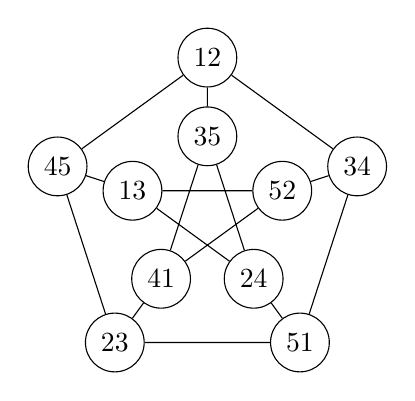
\begin{tikzpicture}
\tikzstyle{every node}=[draw,shape=circle,minimum size=0.5pt];
\node(v1) at (90:2) {$12$};
\node(v2) at (18:2) {$34$};
\node(v3) at (306:2) {$51$};
\node(v4) at (234:2) {$23$};
\node(v5) at (162:2) {$45$};
\node(v6) at (90:1) {$35$};
\node(v7) at (18:1) {$52$};
\node(v8) at (306:1) {$24$};
\node(v9) at (234:1) {$41$};
\node(v10) at (162:1) {$13$};
\draw(v1)--(v2)(v2)--(v3)(v3)--(v4)(v4)--(v5)(v5)--(v1)(v1)--(v6)(v2)--(v7)(v3)--(v8)(v4)--(v9)(v5)--(v10)(v6)--(v8)(v6)--(v9)(v7)--(v9)(v7)--(v10)(v8)--(v10);
\end{tikzpicture}.\]
Petersen graph has girth 5.
\end{example}

\begin{proposition}
An edge is a cut-edge if and only if it belongs to no cycle.
\end{proposition}

\begin{exercise}{1.1.14}

\end{exercise}


\end{document}